%Copyright 2014 Jean-Philippe Eisenbarth
%This program is free software: you can
%redistribute it and/or modify it under the terms of the GNU General Public
%License as published by the Free Software Foundation, either version 3 of the
%License, or {at your option} any later version.
%This program is distributed in the hope that it will be useful,but WITHOUT ANY
%WARRANTY; without even the implied warranty of MERCHANTABILITY or FITNESS FOR A
%PARTICULAR PURPOSE. See the GNU General Public License for more details.
%You should have received a copy of the GNU General Public License along with
%this program.  If not, see <http://www.gnu.org/licenses/>.

%Based on the code of Yiannis Lazarides
%http://tex.stackexchange.com/questions/42602/software-requirements-specification-with-latex
%http://tex.stackexchange.com/users/963/yiannis-lazarides
%Also based on the template of Karl E. Wiegers
%http://www.se.rit.edu/~emad/teaching/slides/srs_template_sep14.pdf
%http://karlwiegers.com
%\documentclass[letterpaper,10pt]{article}
\documentclass[onecolumn, draftclsnofoot,10pt, compsoc]{IEEEtran}
\usepackage{listings}
\usepackage{underscore}
\usepackage[bookmarks=true]{hyperref}
\usepackage[utf8]{inputenc}
\usepackage[english]{babel}
\usepackage{graphicx}
\usepackage{amssymb}
\usepackage{amsmath}
\usepackage{amsthm}
\usepackage{afterpage}
\usepackage{hyperref}

\usepackage{alltt}
\usepackage{float}
\usepackage{color}
\usepackage{url}
\usepackage{setspace}

\usepackage{enumitem}

\usepackage{geometry}

\usepackage{titling}
\usepackage{rotating}
\usepackage{pgfgantt}
\usepackage{graphicx}

\usepackage{xcolor}
\usepackage{anyfontsize}
\usepackage{amsmath}
\usepackage[section]{placeins}
\usepackage[linesnumbered,ruled]{algorithm2e}
\ganttset{group/.append style={orange},
milestone/.append style={red},
progress label node anchor/.append style={text=red}}

\newcommand\blankpage{
    \null
    \thispagestyle{empty}
    \addtocounter{page}{0}
    \newpage}

\geometry{textheight=9.5in, textwidth=7in}
\hypersetup{
    bookmarks=false,    % show bookmarks bar?
    pdftitle={Software Requirement Specification},    % title
    pdfauthor={Jean-Philippe Eisenbarth},                     % author
    pdfsubject={TeX and LaTeX},                        % subject of the document
    pdfkeywords={TeX, LaTeX, graphics, images}, % list of keywords
    colorlinks=true,       % false: boxed links; true: colored links
    linkcolor=blue,       % color of internal links
    citecolor=black,       % color of links to bibliography
    filecolor=black,        % color of file links
    urlcolor=purple,        % color of external links
    linktoc=page            % only page is linked
}%

% 1. Fill in these details
\def \CapstoneTeamName{		Deep Learning on Embedded Platform}
\def \CapstoneTeamNumber{		14}
\def \GroupMemberOne{			Christopher Johnson}
\def \GroupMemberTwo{			Gabe Morey}
\def \GroupMemberThree{			Luay Alshawi}
\def \CapstoneProjectName{		AI Gaming}
\def \CapstoneSponsorCompany{	NVIDIA}
\def \CapstoneSponsorPerson{		Mark Ebersole}

\def \DocType{	%Problem Statement
				%Requirements Document
				%Technology Review
				Design Document
				%Progress Report
				}

\newcommand{\NameSigPair}[1]{\par
\makebox[2.75in][r]{#1} \hfil 	\makebox[3.25in]{\makebox[2.25in]{\hrulefill} \hfill		\makebox[.75in]{\hrulefill}}
\par\vspace{-12pt} \textit{\tiny\noindent
\makebox[2.75in]{} \hfil		\makebox[3.25in]{\makebox[2.25in][r]{Signature} \hfill	\makebox[.75in][r]{Date}}}}

\begin{document}
\begin{titlepage}
    \pagenumbering{gobble}
    \begin{singlespace}
    	% \includegraphics[height=4cm]{coe_v_spot1}
        \hfill
        % 4. If you have a logo, use this includegraphics command to put it on the coversheet.
        %\includegraphics[height=4cm]{CompanyLogo}
        \par\vspace{.2in}
        \centering
        \scshape{
            \huge CS Capstone \DocType \par
            {\large\today}\par
            \vspace{.5in}
            \textbf{\Huge\CapstoneProjectName}\par
            \vfill
            {\large Prepared for}\par
            \Huge \CapstoneSponsorCompany\par
            \vspace{5pt}
            {\Large\NameSigPair{\CapstoneSponsorPerson}\par}
            {\large Prepared by }\par
            Group\CapstoneTeamNumber\par
            % 5. comment out the line below this one if you do not wish to name your team
            \CapstoneTeamName\par
            \vspace{5pt}
            {\Large
                \NameSigPair{\GroupMemberOne}\par
                \NameSigPair{\GroupMemberTwo}\par
                \NameSigPair{\GroupMemberThree}\par
            }
            \vspace{20pt}
        }
        \begin{abstract}
        	In this document we describe the design of a deep learning system developed to learn how to play the arcade game Galaga.
		Galaga is an arcade shooter which was released in 1981 by Namco [1].
		This system is designed with the ultimate goal of being turned into a course for the NVIDIA Deep Learning Institute.
		The documentation will outline exactly what hardware will used, how the system will be put together, and what methods will be used in a way that allows others to recreate this project.
        \end{abstract}
    \end{singlespace}
\end{titlepage}

\newpage
\pagenumbering{arabic}
\tableofcontents

\section{Overview}

\subsection{Purpose}

The main aim of this document is to give others a thorough enough understanding of the project and its design to replicate the project.
The reader of this document should walk away able to understand how the system works and why it was designed this way.
The document must be thorough enough for NVIDIA to recreate the project and package the design into a training course on deep learning.
\newline
\newline
This project is to be used to produce a training course for NVIDIA's Deep Learning Institute.
After the project is complete it will be handed off to NVIDIA for the purposes of accomplishing this goal.
To that end the documentation has been designed to provide readers a clear path towards building this system themselves.

\subsection{Scope}

This document outlines the design of a system for teaching a deep learning neural network how to play the game Galaga.
The sections of this document will outline the system details, setup, and all things necessary to understand how and why the project is designed.
Hardware required, API's to be used, and setup will be detailed as part of the project design.

\subsection{Context}

This system is not designed for an average computer user.
This system is a showcase of possibilities when working with Neural Networks.
As such, no real UI will be developed for the purposes of this project.
Average people may see the result of the final project by viewing the network play Galaga.
\newline
\newline
This system is designed for developers.
Developers should be able to do a project like this as an introduction to deep learning neural networks.
The documentation provided here reflects this focus and is written with developers in mind.

\subsection{Summary}

The neural network created for this project will be able to play Galaga.
Its design is based on SSD, a convolutional neural network designed in coordination with Google Inc.,  University of North Carolina Chapel Hill, and University of Michigan, Ann-Arbor[2].
This neural network will undergo two main phases of training.
One training phase will be done with just still images, while the second will involve live image feed from the game Galaga.
The system will run inference on the Jetson TX1 developer kit, which will interface between a seperate computer via communications scripts written in python.
The Jetson will be linked to the seperate PC via ethernet cable.
Cloud computing GPUs will be used to handle portions of the training.
In total, the system should be able to learn how to play Galaga, and then continually improve as it plays.

\subsection{References}

[1] F. Rojas, "Galaga (Namco)," in gaminghistory101.com, Gaming History 101, 2012. [Online]. Available: https://gaminghistory101.com/2012/03/22/galaga/.\newline
[2] W. Liu et al., “SSD: Single Shot MultiBox Detector,” arxiv.org, 29-Dec-2016. [Online]. Available: https://arxiv.org/pdf/1512.02325.pdf.\newline

\subsection{Definitions}
\begin{description}

  \item[Neural Network:] A multilayered graph structure containing nodes, referred to as neurons, and weights that affect how likely the node is to be chosen when confronted with a decision.
The weights of nodes are decided through training the network, and a traversal of the graph acts as a large chain of decisions as the neural network is confronted with situations.

  \item[Deep Learning:]  Using a layered neural network constructed by GPU processing to teach a computer how to accomplish a specific task.

  \item[Convolutional Neural Network:] A neural network specifically designed to take images as input.
It uses convolutional layers to process the image into a more manageable chunk of data and extracts the information relevant to the network.

  \item[Caffe:] A code framework that allows for complex mathematical operations that are required for training a neural network.

  \item[API:] Application Programming Interface

  \item[Jetson TX1:] Quad core embedded system designed for power efficiency and deep learning projects

  \item[OS:] Operating system

  \item[OpenCV:] (Open Source Computer Vision) is a library that can be used with different languages(C, C++, Java, Python, etc.). It provides standard functionalities such as image capture, Faces recognition, Gesture recognition, Motion tracking, Mobile robotics, Object identification and Image manipulation.

  \item[Galaga:] Galaga is an arcade video game released in 1981 by Namco [1]. The player takes control of a small space ship and must shoot at and dodge waves of alien space ships.
Victory in a level is achieved by destroying all enemy ships.

\end{description}

\section{Design}

\subsection{Introduction}

This section lays out several viewpoints from which we have approached the design of this project.
Each component will be matched under an appropriate viewpoint that gives the reader a clear idea of how the design was apparoached.
Each subsection details a different set of components, many of which will be lumped together, which constitute a major piece of the final design.
There are three main viewpoints from which we have approached the design:
\begin{itemize}
  \item Structure Viewpoint: Design elements approached from a structural level.

  \item Information Viewpoint: Design elements approached from a perspective of data flow operations and data processing.

  \item Interaction Viewpoint: Design elements relevant to getting systems to integrate with each other. Particularly focused on hardware setups required for the rest of the process.
\end{itemize}

Each viewpoint is covered in more depth in its respective section.

\subsection{Structure viewpoint}%Gabe

This section covers integral structural elements of the system and how they come together.
Tools used will be covered to give readers an idea of how we set up the system structure.
The heart of this structure is our neural network set-up.

\subsubsection{Neural network setup}%Gabe

The neural network set-up itself is a multi-layered combination of components.
At the basic level of design, our neural network follows the architecture known as SSD.
SSD is designed, as a convolutional neural network, specifically to process images and categorize objects within the images in real time.
The network uses a set of bounding boxes and feature maps created through layers of network code to identify individual components of a frame [2].
A basic visualization of this detection style can be seen in \ref{fig:4.1}.
\newline
\newline
\begin{figure}
  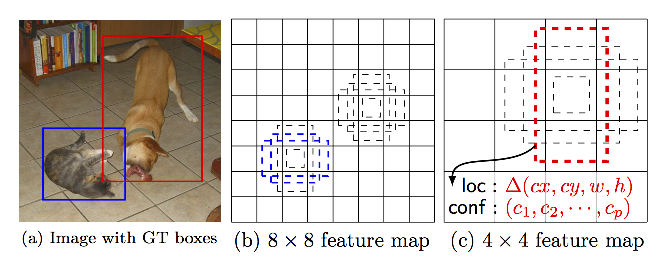
\includegraphics{SSDBoxes.eps}
  \caption{SSD Image Mapping}
  \label{fig:4.1}
\end{figure}The network set-up provided by SSD is built using the deep-learning framework Caffe, so its functions are intimately involved in the final project.
Caffe allows for command line instructions to be sent to define the network.
To set up the network and Caffe properly we are using the tools provided by Caffe itself and the components found in the SSD branch of the main Caffe repository on Github.
\newline
\newline
Training of the neural network will be done on NVIDIA GPUs on the Amazon Web Services cloud as well as on normal PC's.
Cloud computing is mostly used in the later stages to speed up the training process.
Once the network is fully trained, it will be deployed on the Jetson to play the game Galaga in real time.
\newline
\newline
The structural goal of the neural net changes between two stages.
In the first stage, the structure of the neural net is meant purely to teach it how to recognize and categorize in game objects from images.
In the second stage, the neural network will be deployed on the Jetson TX1 and will take active game information.
It will use that information to make one of four choices: move left, move right, stop, or shoot.
More detail on the training will be given in section \ref{sssec:num2}.

\section{Information viewpoint}\label{sssec:num2}%Luay

The data in this section consists of image processing of the game being played as well as the trained neural network.
This section will go in depth of both how image processing will be done as well as different ways to train and improve the neural network.
A pseudocode will be included to give an overview of where these data will be used in this project.
Also, the pseudocode in \ref{sssec:num3} will include a general algorithm to show how output decision's layer works.

\subsection{Set up image dataset}%Luay

Setting up image set for training and testing requires using annotation methods that can be used to label and identify objects from any given image.
In this project, Pascal VOC annotation is being used because it's the most common and supported by the majority of deep learning frameworks as well as neural networks.
The deep learning framework we are currently using supports Pascal VOC and Coco but only Pascal VOC is being used.
However, in order to prepare the annotations we would need to separate train validation images and test images so we can easily list them in a text file along with their path and XML which is the annotation file.
In addition, we would need to write down a label map file that lists all the objects that need to be identified by the neural network.
Overall, the files are needed in order to create the LMDB database are trainval.txt, test_name_size.txt, test.txt, lebelmap_voc.prototxt.
Examples of how to write those files are in \ref{sssec:num33}.
\subsection{Neural training methods}%Gabe

The training of the neural network will be done in two stages.
In the first stage, we will be using images created from the game to teach the network how to recognize in game objects.
Given that GoogLeNet was designed with image categorization in mind, this set-up will be easy to create and bring to functionality.
We will feed the network with images doctored by OpenCV and it will interpret them and label them.
Once it has a high degree of success in correctly identifying in game objects, we will take the training to stage two.
\newline
\newline
In the second stage of training we will be feeding the network images directly from live game progress.
The game will be running and the network will be deployed on the Jetson.
The network will be given the ability to take actions based on the objects it identifies on screen.
Positive feedback will be given to the neural network when it correctly kills an enemy or completes a level.
Negative feedback will be given to the network when it dies, gets a game over, or loops too long doing nothing.
As the neural network plays the game, it will improve performance and eventually be considered proficient.

\subsection{Input image processing}%Luay

After having a trained neural network, a software written in python will start by loading the necessary dependencies, which are OpenCV.
Then, a video capture of the game will take a place to record the monitor where the game is being played using OpenCV's API.
The hardware connection of the camera, as well as the control mechanism of the game, shall be explained in section \ref{sssec:num1}.
Since videos are just consecutive images, OpenCV will be used to get each frame and then pass the image to the input of neural network.
Then we would need to do a forward call to the network's API using Caffe which give us the output from the neural network.

\subsection{Data visualization}%Chris

It was necessary to figure out how to display the results of each round.
We decided it would be best to have a summary, graphical display of the data at the end of the playthrough.
Once the program runs out of lives, a screen will appear, graphing statistics about the machine's performance.
These statistics will include things such as how long the machine lasted, how many levels it completed, which enemies or objects took away the most lives, and so on.
Having detailed and easily readable data is key to knowing how to train the machine to keep performing better in the game.


\newpage

\subsection{Setup Image Data Sets Example}\label{sssec:num33}

\subsubsection{trainval.txt}
train/image1.png train/image1.xml

\subsubsection{test.txt}
test/test1.png test/test1.xml

\subsubsection{test_name_size.txt}
imageName imageWidth imageHeight\newline
test1     1080       1920

\subsubsection{labelmap_voc.prototxt}
\{\newline
name:"player",\newline
label: 0,\newline
display_name:"player"\newline
\}\newline
\textbf{Note:} Label is a numerical value and should be incremented every time a new label is added.

\subsection{Pseudocode}\label{sssec:num3}
% \subsection{Decision Layer Pseudocode}\label{sssec:num300}
\begin{algorithm}
  % Load necessary packages for openCV, and Caffe.\.
  % Load the trained net.\.
  % Convert the trained net to an object which OpenCV understands.
  % Start video capture.
  % For each frame in the video capture:
  \emph{Reshape the Layer to set output one thing of size 1 - for possible outputs such as left,right,shoot}\;
  \emph{In Forward Function:};\newline
  \nl$player_x,player_y\leftarrow Coordinates Of the label Player$\;
  \nl$topData\leftarrow buttom[0]->date()$\;
  \ForEach{object on the game}{
    \If { (object.y $\geq$ 300) and and (object.x $\leq$  player_x+200) }
    {
      \nl$topData[0]\leftarrow 0$\;
    }
    \ElseIf{ (object.y $\geq$ 300) and (object.x $\leq$  player_x+200) }
    {
      \nl$topData[0]\leftarrow 1$\;
    }
    \ElseIf{ (object.x $\leq$  player_x+100) and (object.x $\geq$  player_x-100) }
    {
      \nl$topData[0]\leftarrow 2$\;
    }
  }

    \caption{Decision Layer}
\end{algorithm}

\begin{algorithm}
  % Load necessary packages for openCV, and Caffe.\.
  % Load the trained net.\.
  % Convert the trained net to an object which OpenCV understands.
  % Start video capture.
  % For each frame in the video capture:
  \emph{Load necessary packages for openCV, and Caffe}\;
  \emph{Load the trained net and label map}\;
  \emph{Do input preprocessing using Caffe Transformer API}\;
  \emph{Start video capture}\;
  \ForEach{frame in the video capture}{
    \emph{Load the frame to data layer which is the input of the nerual network}\;
    \emph{Call Caffe forward API to get decision output from the network}\;
    \emph{Send the decision through the network to the game hosted computer with a command such as left, right and shoot}\;
  }

    \caption{Jetson TX1 plays Galaga}
\end{algorithm}

\section{Interaction Viewpoint}\label{sssec:num1}%Chris

This section details how our physical hardware components interact to form a cohesive system.
It will outline several pieces of hardware used to realize the goal of playing galaga.

\subsection{Hardware setup}%Chris

While working with the Jetson TX1 there are several things that we needed to decide.
These included our methods to communicate with our client, and the hardware used with the Jetson.
Choosing out hardware was key to determining how each piece would fit into the design.
\newline
\newline
Our project will actually need to be able to control the game.
Inputs from the neural net need to be received by the game so that it can be played.
To do this we decided not to use the standard keyboard.
Using a keyboard requires a lot of additional coding to map the Jetson to the controls.
We had originally decided that we would use a gaming controller and wire the Jetson to it so that the neural net could send the game commands.
A game controller would have significantly reduced the work load because it would have already contained a lot of built in functionality that we needed to connect it to the Jetson.
However instead of requiring another piece of hardware we decided to just use Windows APIs and a client server system.
The Jetson will be able to send commands to the game through an ethernet cable.
This setup is outlined in figure \ref{fig:4.2}.
\newline
\newline
\begin{figure}
  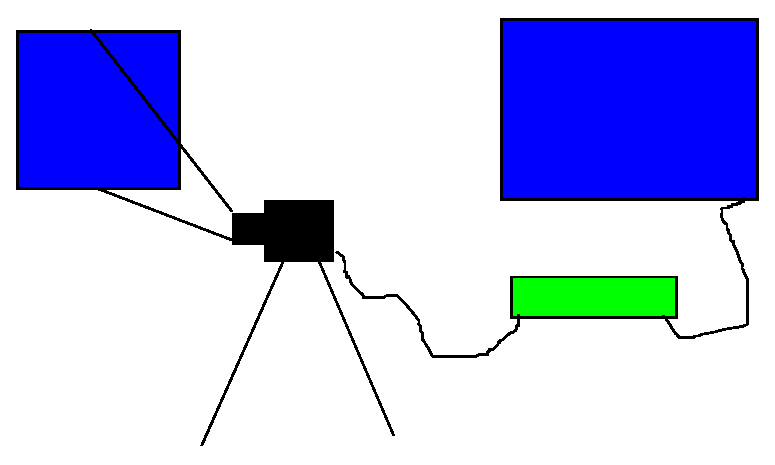
\includegraphics[width=\textwidth]{design.eps}
  \caption{Hardware Layout}
  \label{fig:4.2}
\end{figure}% Figure \ref{fig:4.3} shows the basic layout.
Since the Jetson has to learn how to play the game on its own it needs to be able to see the game.
By see I mean that video has to be captured and translated into data the neural net can understand.
We were able to buy a pretty inexpensive camera that could capture more than enough detail.
It only cost about \$25.
This option had not been in the tech review originally but after some work on the project we realized that in order for the neural net to play the game it didn't need incredibly high quality images.
The neural net only needed images where it was obvious to see what enemies were being recorded.
Also to react to the game quickly enough to beat the first level we realized the neural net wouldn't have to process more than 30 frames per second.
The camera will be connected to the Jetson and aimed at the monitor, which is connected to the computer running the game.
The program will first be trained by being given the video input to recognize and characterize objects within the game.
We will set up tables so that the neural net will be able to store information such as the locations of objects.
Once the objects and tables are set up the neural net will be able to train itself by playing the game, sending commands through an ethernet cable.
Its decisions will be based on the table of information that it stores and will increasingly be able to survive the game longer.
Eventually the neural net will learn to respond to certain patterns in the table in order to become better at the game.

\section{Conclusion}
The goal of this design document is to provide the how to of this deep learning project which will be turned to the NVIDIA's deep learning institute to use it in a deep learning course.
The overall steps for this document are to teach the Jetson TX1 to play the game Galaga by training a neural network to identify game objects and become effectively able to move the player away from enemies.
This can be done based on three major phases which are preparing images for the game objects, training a neural network based on the set of images with labels, and finally by using a camera connected to the Jetson TX1 while the game hosted on a different machine that is being controlled using the Jetson TX1 and a controller input.

\end{document}
